\chapter{Develop your own analysis}\label{chap:DevelopNewAnalyses}

This chapter explains step-by-step how to develop and run your own Harmony analyses.

\screecast{http://youtu.be/iQCeLmu2WDg}

%\section{Run Harmony}\label{sec:RunInEclipse}
%
%	\begin{itemize}
%		\item Go to \texttt{File $\rightarrow$ Import}
%		\item Select \texttt{Launch Configurations} under the \texttt{Run/Debug} category and click on \texttt{Next}
%		\item Click on \texttt{Browse} to select the \emph{configuration} directory located in the \emph{HarmonyWorkingDirectory}
%		\item Select the file \emph{Harmony.launch} as shown in figure \ref{} and click on \texttt{Finish}
%		
%	\end{itemize}
%
%Eclipse uses \emph{Run configurations} in order to know what should be launched and how : which plugins, which execution environment,... A default \emph{Run configuration} is provided in the \texttt{harmony.core} plug-in. In order to use it you have to import the \texttt{harmony.core} plug-in from your Eclipse installation into your workspace. 
%
%You can do this via the \texttt{File $\rightarrow$ Import} menu. Then select \texttt{Plug-ins and Fragments} (see figure \ref{fig:coreBundleImportMenu}). 
%
%In the \texttt{Import Plug-ins and Fragments} wizard, select \texttt{Import As $\rightarrow$ Project with source folders} as shown in figure \ref{fig:coreBundleImportMenu}.
%
%	\begin{figure}[H]
%		\centering
%		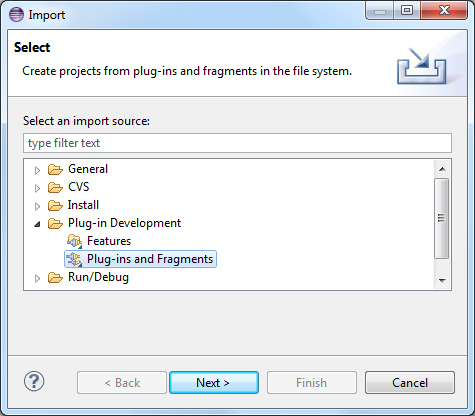
\includegraphics[width=.49\linewidth]{import-menu}
%		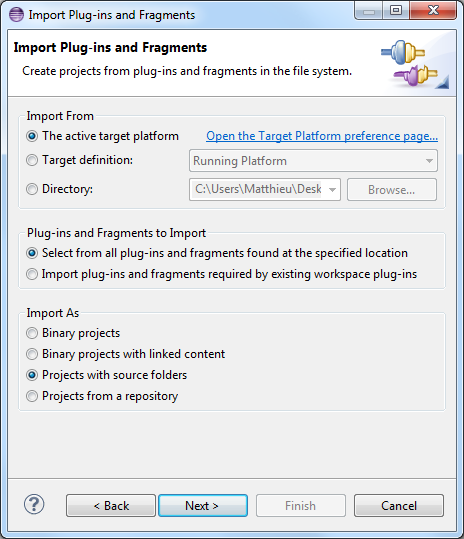
\includegraphics[width=.49\linewidth]{import-plugin-menu}
%		\caption{Menu for the importation of plugins in the workspace}
%		\label{fig:coreBundleImportMenu}
%	\end{figure}
%
%In the next step, add the \emph{fr.labri.harmony.core} plug-in in the list of \emph{Plug-ins and Fragments to Import}. You may use the filter box with "fr.labri" in order to find more rapidly the \emph{fr.labri.harmony.core} plug-in as demonstrated in figure \ref{fig:coreBundleImportSelection}.
%
%	\begin{figure}[H]
%		\centering
%		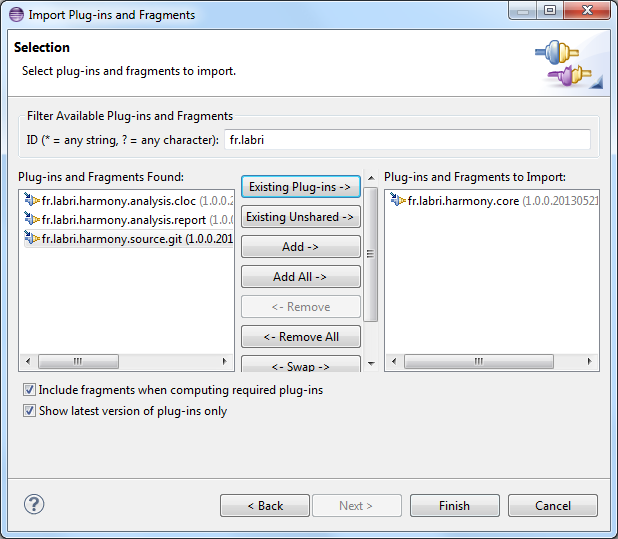
\includegraphics[width=.8\linewidth]{import-plugin-selection}
%		\caption{Selection of the Harmony core plugin for importation}
%		\label{fig:coreBundleImportSelection}
%	\end{figure}
%
%Finally press \texttt{Finish}. A new project has been added to your workspace. You may have build errors, in such a case you need to clean the project via the \texttt{Project $\rightarrow$ Clean} menu.
%
%We will be able to run Harmony in a few steps. The next thing to do is to copy the \texttt{configuration} directory --located in the \texttt{resources} directory from the \texttt{fr.labri.harmony.core} plugin-- into the root of workspace, where you should have a \texttt{.metadata} directory and the plug-in you imported:\\
%
%\begin{lstlisting}[language=bash]
%drwx------+ 1 XXXXXX None 0 21 mai   11:27 .metadata/
%drwx------+ 1 XXXXXX None 0 21 mai   14:09 configuration/
%drwx------+ 1 XXXXXX None 0 21 mai   13:08 fr.labri.harmony.core/
%\end{lstlisting}
%
%
%Then go back into Eclipse, and open the \texttt{Run Configurations} window (via the \texttt{Run} menu). In the left menu, you should see an \texttt{HarmonyEquinox} configuration under the \texttt{OSGi Framework} node as shown in figure \ref{fig:run-configurations}. Select it.
%
%You can now see a list of plugins. The ones that are selected are the ones that will be loaded if you launch this \emph{Run configuration}. Now, uncheck the "Show only Selected" checkbox (on the right) and type "fr.labri" in the filter box located at the top of the plugins list. Add the harmony plugins that are not imported in your workspace (i.e. reporting, cloc, and source.git) as shown in figure \ref{fig:run-configurations}. Remember that if you develop new analyses, you must update your \emph{Run configuration} by adding the new plugin otherwise you will not be able to run your analysis.
%
%	\begin{figure}[H]
%		\centering
%		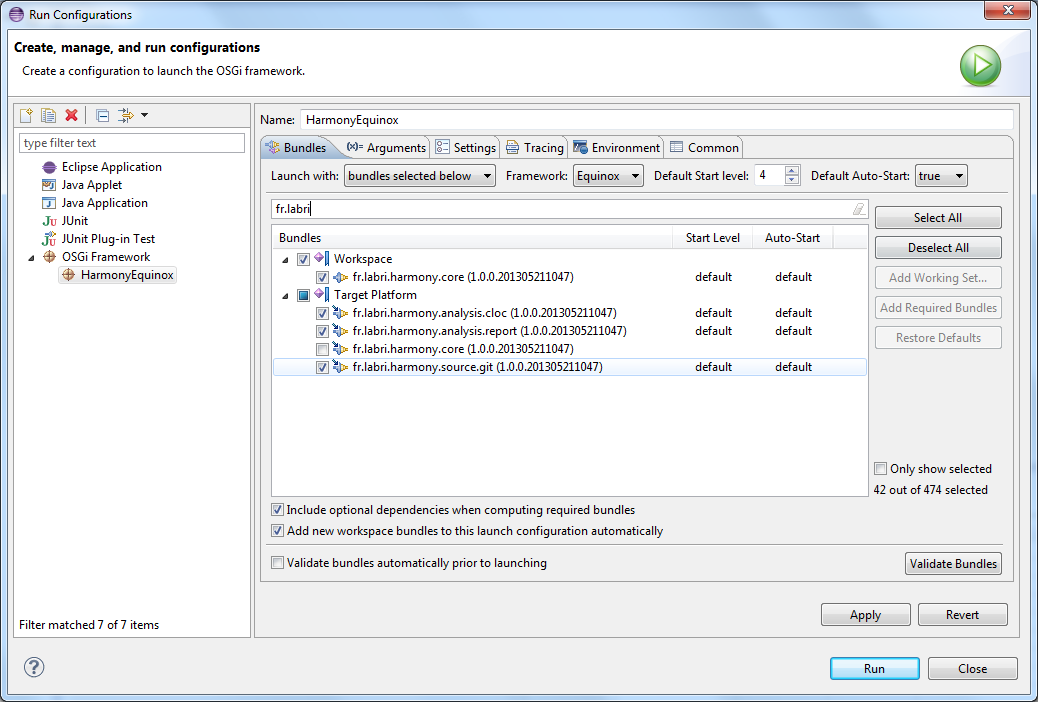
\includegraphics[width=.85\linewidth]{run-configurations}
%		\caption{Set up of the run configuration}
%		\label{fig:run-configurations}
%	\end{figure}
%
%Finally you can hit \texttt{Run} to launch the selected plugins. Once the OSGi console is loaded, type \texttt{harmony} (see figure \ref{fig:run-harmony}.
%
%	\begin{figure}[H]
%		\centering
%		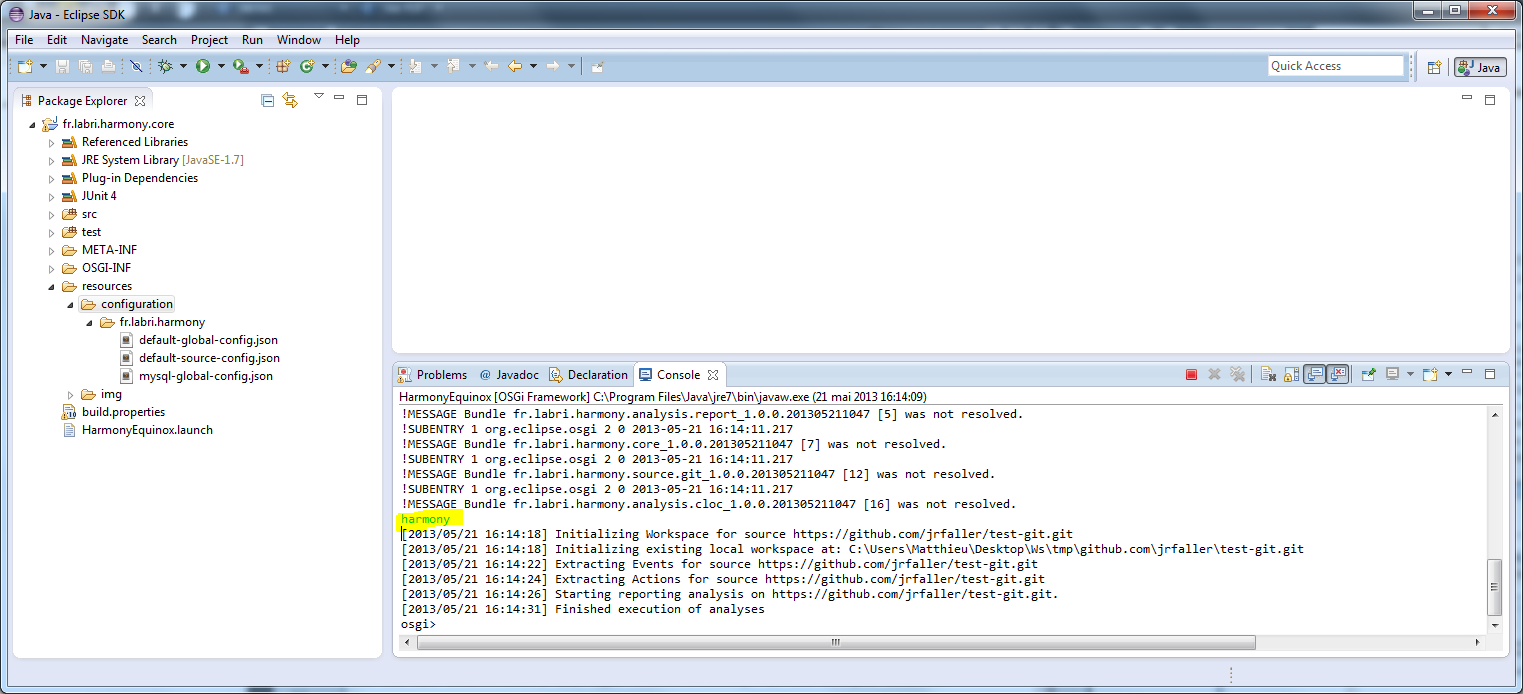
\includegraphics[width=.95\linewidth]{run-harmony}
%		\caption{OSGi console with Harmony running}
%		\label{fig:run-harmony}
%	\end{figure}


%\section{Create a new analysis}
%
%Now that your development environment is ready and that you know how to run analysis within Eclipse. We will see how you can create your own analysis. There are two ways of doing so, the easy way by using the dedicated wizard (see section \ref{newAnalysis:wizard}) and the hard way by creating the project from scratch (see section \ref{newAnalysis:fromScratch}). In both cases do not forget to add your new analysis to your \emph{Run Configuration} (see previous section).

\section{New analysis wizard}\label{newAnalysis:wizard}

	\begin{itemize}
		\item Go to \texttt{File $\rightarrow$ New $\rightarrow$ Project...}
		\item Select \texttt{Analysis} under the \texttt{Harmony} category and click on \texttt{Next} 
		\item Fill out the form (see Figure \ref{fig:wizard-new-analysis-form})
			\begin{itemize}
				\item \emph{Project name}: this name must follow the Java package naming convention as the project name will be used as your root package as well as your plugin unique identifier.
				\item \emph{Analysis class name}: name of the class that will implement the analysis.
				\item \emph{Database facilities}: we will not need that for the moment.
			\end{itemize}
		\item Click on \texttt{Finish}
	\end{itemize}

	\begin{figure}[H]
		\centering
		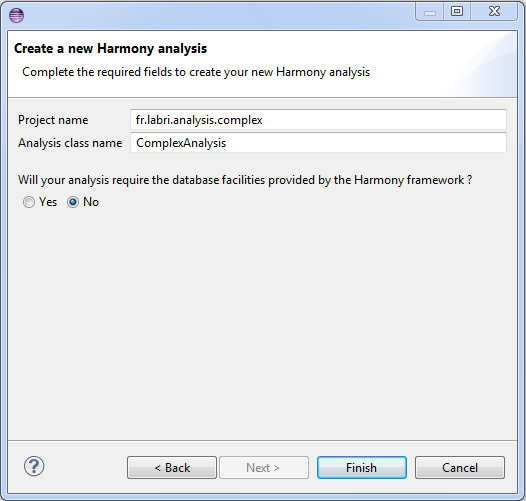
\includegraphics[width=.7\linewidth]{wizard-new-analysis-form}
		\caption{Form for creating a new analysis}
		\label{fig:wizard-new-analysis-form}
	\end{figure}

\section{Implement your analysis}

	\begin{itemize}
		\item Implement your analysis in the method \emph{runOn(Source src)} located in your analysis class.
		\item Modify the general configuration file : \emph{default-global-configuration} to indicate the name of your new analysis (see Chapter \ref{chap:configuration} for more explanation).
		\item Run the OSGI console based on the Harmony \emph{Run Configuration} (see Figure \ref{fig:run_harmony})
		\item Type \texttt{harmony} in the OSGi console and press Enter.
	\end{itemize}

	\begin{figure}[H]
		\centering
		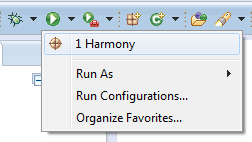
\includegraphics[width=.4\linewidth]{run_harmony}
		\caption{Harmony launching}
		\label{fig:run_harmony}
	\end{figure}

	
	




%
%\section{How to write an analysis}
%
%	\subsection{The Harmony model}
%	
%		\begin{figure}[H]
%			\centering
%			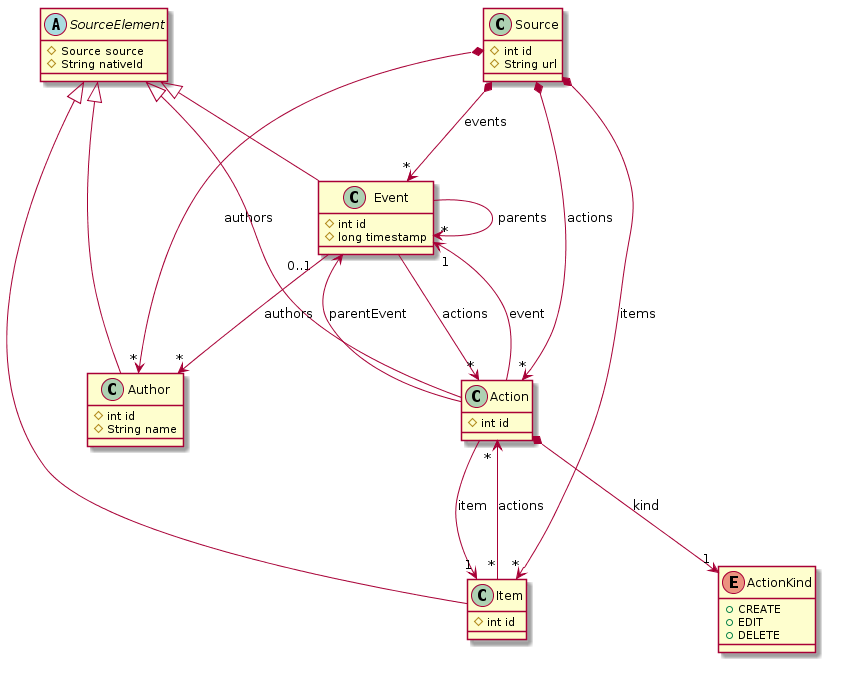
\includegraphics[width=\linewidth]{data-model}
%			\caption{Class diagram of the main concepts of the Harmony generic data model}
%			\label{fig:data-model}
%		\end{figure}
%	
%	\subsection{Using the database}
%	
%	\subsection{Output management}
	
% TODO explain the use of the dao
%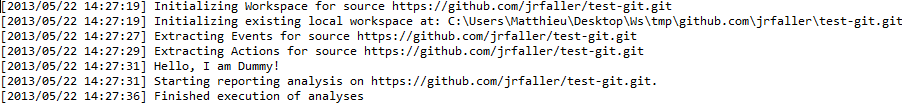
\includegraphics[width=6in]{dummy-execution}
%
%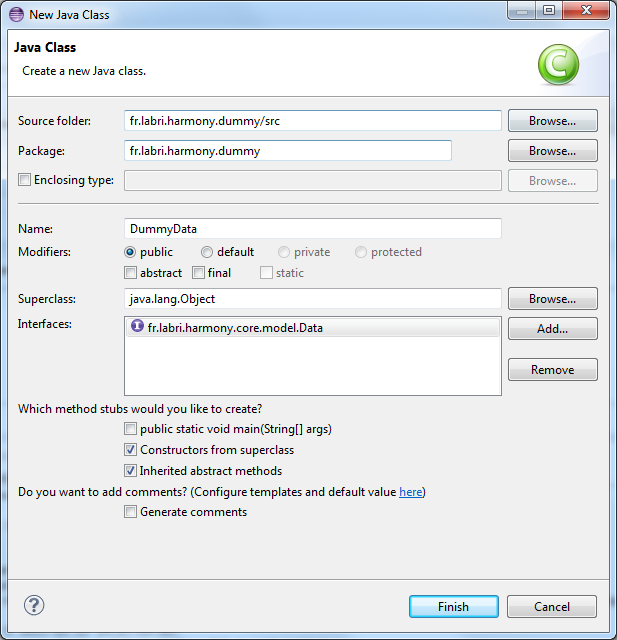
\includegraphics[width=6in]{new-data-class}
%
%
%\begin{lstlisting}[language=Java]
%DummyData d = new DummyData();
%d.setContent("plop");
%dao.saveData(this, d, Data.SOURCE, src.getId());
%\end{lstlisting}




